\chapter{Applicazione per la visualizzazione dei dati del magazzino}\label{sec:1Applicazione}
In questo capitolo si descrive la prima applicazione sviluppata presentando i requisiti, la progettazione, lo sviluppo e i test.\\
\\L'applicazione per i dati del magazzino ha lo scopo di agevolare gli operatori nella visualizzazione delle informazioni di un articolo. I dati recuperati dal \glossario{ERP} aziendale collocato su server con \glossario{OS400} come sistema operativo vengono resi visualizzabili da un'applicazione per qualsiasi dispositivo mobile non dovendo più necessariamente usare il computer.\\
Per sviluppare questa applicazione sono stati utilizzati i seguenti strumenti, descritti nel capitolo dedicato alle tecnologie:
\begin{itemize}
    \item Power Apps;
    \item DB2;
    \item Microsoft SQL.
\end{itemize}

\newpage

\section{Analisi dei Requisiti}\label{sec:1App-Requisiti}
Nella \tablename \space \ref*{tab:Requisiti-M} sono presentati i requisiti dell'applicazione per la visualizzazione dei dati del magazzino.
\renewcommand{\arraystretch}{1.5} %ampiezza righe
\begin{table}[H] % in caso di longtable per il cambio pagina, commentare H, e il \begin{tabular} spostando dopo longtable quanto scritto dopo tabular {|5em|10em|....}
  \begin{tabular}{ |m{6em}|m{28em}| }
    \hline
    \textbf{Codice} & \textbf{Descrizione requisito} \\
    \hline
    \textbf{RFO01-M} & Applicazione sviluppata per smartphone e tablet \\
    \hline
    \textbf{RFO02-M} & Sincronizzazione frequente con il sistema aziendale \glossario{ERP} \\
    \hline
    \textbf{RFO03-M} & La lettura del codice articolo tramite scannerizzazione \\
    \hline
    \textbf{RFO04-M} & Elenco delle informazioni obbligatorie da visualizzare:
          \begin{itemize}
          \begin{spacing}{1.1}
            \item descrizione dell'articolo;
            \item giacenza totale;
            \item quantità ordinata;
            \item quantità scaffale;
            \item operatore che acquista;
            \item fornitore;
            \item messaggio;
            \item tipo di locazione;
            \item locazione.
          \end{spacing}
          \end{itemize}\\
    \hline
    \textbf{RFD05-M} & Elenco delle informazioni desiderabili da visualizzare:
          \begin{itemize}
          \begin{spacing}{1.2}
            \item scorta minima;
            \item giacenza specifica per locazione.
          \end{spacing}
          \end{itemize} \\
    \hline
    \textbf{RVO01-M} & Applicazione sviluppata in ambiente Microsoft con \glossario{Power Apps} \\
    \hline
    \textbf{RQO01-M} & Ricevere la risposta dal database entro 5 secondi \\
    \hline
    \textbf{RQD02-M} & Applicazione sviluppata in un'unica schermata \\
    \hline
  \end{tabular}
\caption{Classificazione requisiti dell'applicazione dati del magazzino}
\label{tab:Requisiti-M}
\end{table}

\section{Progettazione}\label{sec:1App-Progettazione}
Il sistema aziendale \glossario{ERP} è basato su database \glossario{DB2} che si trovano sui server aziendali in Inghilterra.
Sono macchine \glossario{IBM AS400} con il sistema operativo OS400, un sistema ad oggetti nato negli anni ottanta che offre un altissimo grado di affidabilità usando la tecnologia RAID5\footnote{anche in caso di rottura di un disco garantisce il mantenimento dell'integrità delle informazioni.} ed è inataccabile da virus e hacker.
Questo sistema si usa principalmente per la gestione dei database, è molto veloce al suo interno ma un suo svantaggio è la lentezza nell’estrarre i dati dall’esterno. 
Per connettersi dall’esterno si può usare un connettore di tipo \glossario{ODBC} da cui si può creare una vista logica virtuale oppure si esportano i dati che vengono salvati nei server locali; tra questi due server deve essere schedulato un aggiornamento frequente per garantire la correttezza dei dati.\\
Infine Power Apps si connette direttamente al cloud di SQL Server, l’applicazione con un’unica schermata visualizza solo le informazioni relative al codice articolo scansionato. 
Tutti i vari passaggi richiedono l’accesso ai singoli database criptati mediante specifico utente e password per garantire maggiore sicurezza.\\
Si è deciso di usare un’applicazione sviluppata in ambiente Microsoft in quanto in azienda tutti i dipendenti ed operai possiedono il proprio account personale con licenza completa.\\
La seguente \figurename \space \ref*{fig:M-Schema} illustra schematicamente l'idea di progettazione con le relative tecnologie.
\begin{figure}[H]
  \centering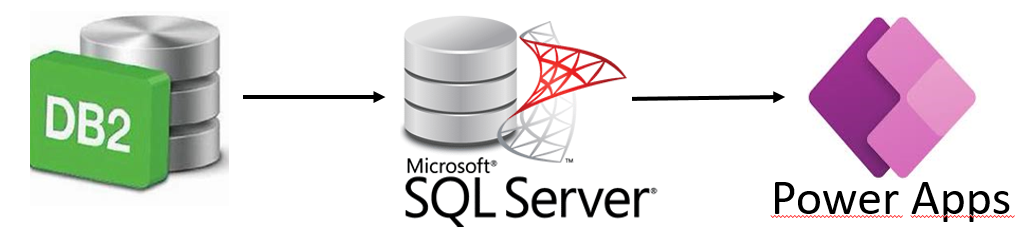
\includegraphics[width=1.0\textwidth, height=1.0\textheight,keepaspectratio]{immagini/M-schema.png}
  \caption{Schema delle tecnologie dell'applicazione per il magazzino}
  \label{fig:M-Schema}
\end{figure}

\section{Sviluppo} \label{sec:1App-Sviluppo}
Nei server aziendali in Inghilterra, al fine di agevolare la successiva estrazione dei dati e visto che effettuare le operazioni direttamente dentro il sistema \glossario{OS400} è molto più rapido, si crea una nuova tabella nel database \glossario{DB2} in cui viene effettuato il \glossario{join} tra le varie origini dei dati, infine si selezionano solo le colonne utili.
Il file ottenuto contiene più di cento mila record ed è già il risultato finale desiderato in cui si vorrebbe effettuare la ricerca del codice articolo per le relative informazioni. 
\\Nelle seguenti Figure \ref*{fig:M-DB2} si illustrano due passaggi dell'estrapolazione delle informazioni necessarie, tramite una macchina virtuale si accede al sistema OS400 così da eseguire le operazioni al suo interno.\\ 
\begin{figure}[H]
  \centering\subfloat[Elenco delle \glossario{query} tra cui è stato fatto il join per ottenere il nuovo file \label{a}]{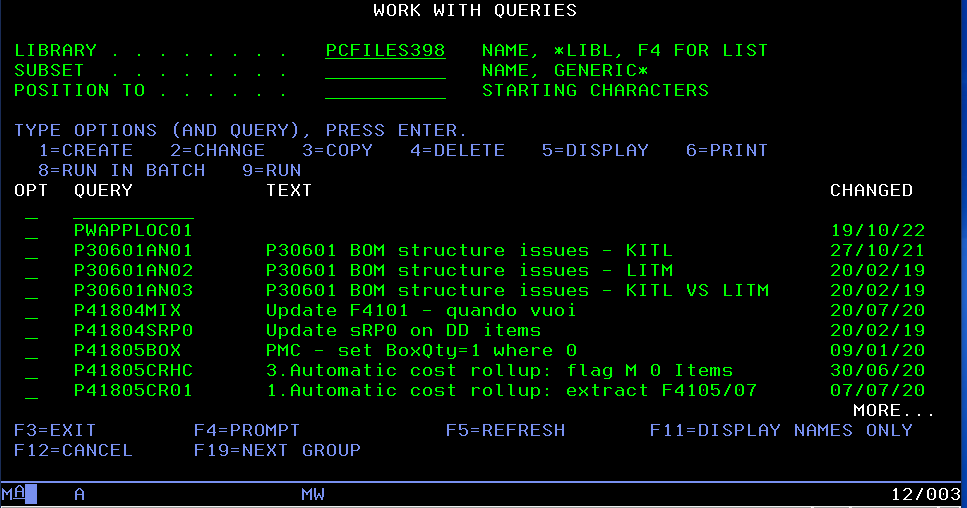
\includegraphics[width=1.0\textwidth, height=1.4\textheight,keepaspectratio]{immagini/M-db2-file.png}}\qquad
  \centering\subfloat[Elenco dei campi all'interno del file \label{b}]{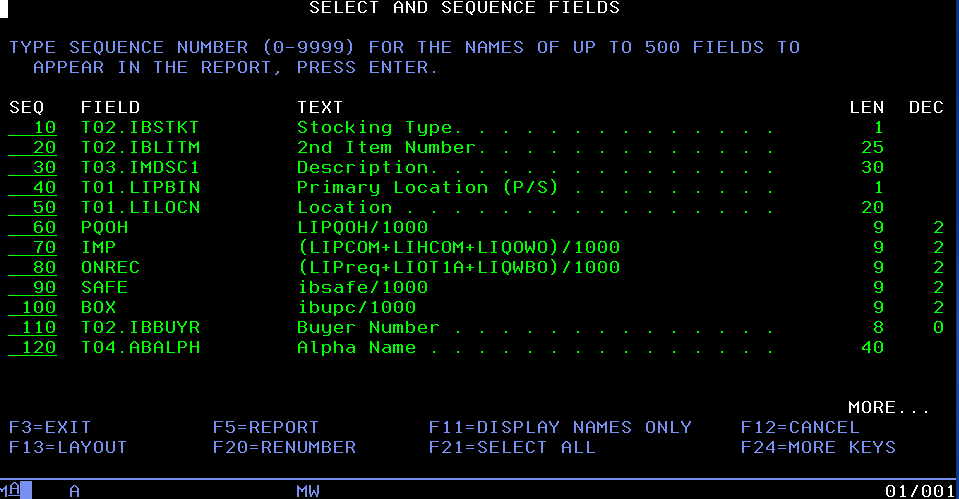
\includegraphics[width=1.0\textwidth, height=1.4\textheight,keepaspectratio]{immagini/M-db2-colonne.png}}
  \caption{Configurazioni del file nel database DB2 per l'applicazione dati del magazzino}
  \label{fig:M-DB2}
\end{figure}
Mediante il connettore \glossario{ODBC} si è creata una connessione \glossario{Linked Server} e tramite il codice scritto in \glossario{Microsoft SQL} si importa la tabella sul server di Padova.\\
Tra i due server è stato schedulato un aggiornamento ogni 15 minuti durante l’orario lavorativo, si veda la \figurename \space \ref*{fig:M-Schedulazione} per la schedulazione.
\begin{figure}[H]
    \centering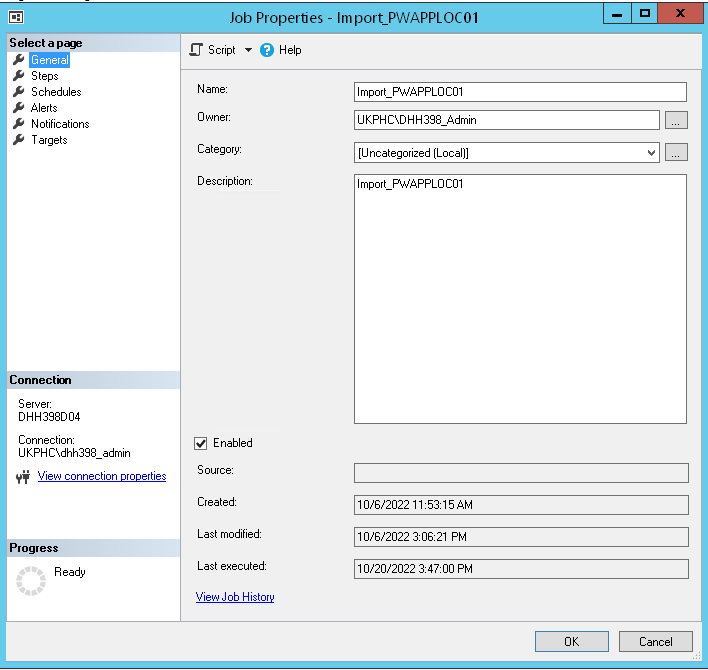
\includegraphics[width=0.8\textwidth, height=0.8\textheight,keepaspectratio]{immagini/M-schedulazione.png}
    \caption{Schedulazione aggiornamento database per l'applicazione dati del magazzino}
    \label{fig:M-Schedulazione}
\end{figure}
Per l’aggiornamento dei dati si è deciso di non aggiornare solo i record modificati ma ogni volta di ripulire il file e poi importare nuovamente tutti i record.
L’eliminazione e la nuova importazione totale è più conveniente dell’aggiornamento dei singoli record in quanto si riduce il rischio di errore, si alleggerisce l’operazione non dovendo fare un continuo controllo tra i due file i quali potrebbero anche non essere ugualmente ordinati e ciò comporterebbe un ulteriore rallentamento.\\
L’applicazione come da richiesta è stata sviluppata in un’unica schermata: oltre alla scannerizzazione e scrittura del barcode, nella parte della si trovano le informazioni da visualizzare mentre nella seconda parte l’elenco delle locazioni specifiche di quell’articolo.
%\\
Nel database più record contengono lo stesso codice articolo e varia solo la locazione e relativa giacenza; quindi, sia per evitare di essere ripetitivi sia per fornire informazioni compatte a vista d’occhio in un’unica schermata, nella prima parte le informazioni vengono visualizzate una sola volta mediante questa formula nel suo contenitore generale:\\
\texttt{FirstN(Filter(Search([@PWAPPLOC01];TextInput1.Text;"IBLITM");\\
        Len(TextInput1.Text)=Len(TrimEnds(IBLITM)));1)
       }\\
\textit{Cerca nel database i record con il campo codice articolo (IBLITM) corrispondente a ciò che è scritto nella cella di input; filtra solo quelli che hanno lunghezza esattamente uguale alla lunghezza del codice inserito nella cella di input (calcolata con la funzione Trim per togliere gli spazi vuoti finali); filtra solo il primo record.}\\
Nella seconda parte per visualizzare l’elenco delle locazioni la formula è uguale ma senza il restringimento al primo record e quindi si filtra un elenco di record. Per la visualizzazione effettiva dei dati sono necessarie singole celle di testo impostate sulla specifica colonna; la \figurename \space \ref*{fig:M-Applicazione} mostra la schermata dell'applicazione
\begin{figure}[H]
    \centering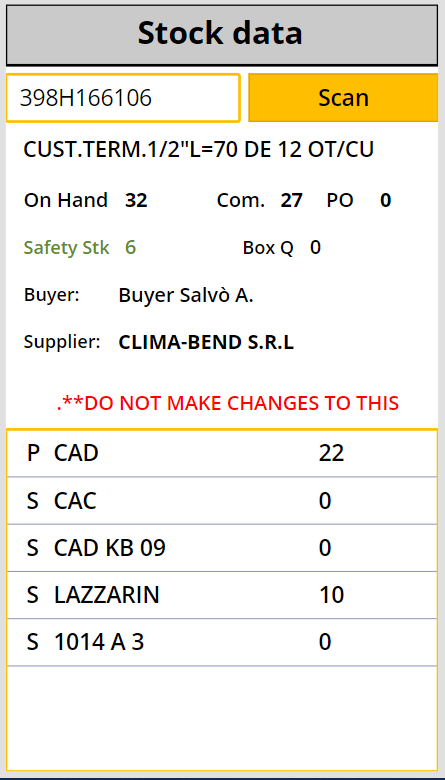
\includegraphics[width=0.5\textwidth, height=0.5\textheight,keepaspectratio]{immagini/M-applicazione.png}
    \caption{Unica schermata dell'applicazione per il magazzino}
    \label{fig:M-Applicazione}
\end{figure}

\newpage
\section{Verifica e Validazione}\label{sec:1App-Verifica}
Per la verifica essendo l'applicazione sviluppata mediante \glossario{Power Apps}, software basato sul principio low-code, risulta difficile effettuare i classici test.
E' stata svolta una minimale analisi statica cioè rilettura sulle formule e impostazioni inserite per configurare gli elementi.
Principalmente si è effettuata analisi dinamica facendo girare l'applicazione ed eseguendo test d'uso anche di casi estremi così da vederne eventuali bug o comportamenti imprevisti.\\
Durante l'analisi dinamica il principale problema rilevato è stato che in presenza di più codici a barre l'applicazione legge e cerca il primo codice a barre decifrato che spesso poi non trova nel database dei codici articolo.
Non si può risolvere lato applicazione perchè i codici articolo sono di più tipologie e lo scanner di \glossario{Power Apps} prevede tipo codice automatico o solo un tipologia selezionabile (non è possibile indicare una lista di più tipologie).
Andrebbe risolto con maggior ordine nelle etichette e nel loro posizionamento, oppure in azienda utilizzare sempre la stessa tipologia di codice a barre per i codici articolo e magari una diversa per i codici legati al numero d'ordine o alla spedizione.\\
La validazione dell'applicazione è stata effettuata insieme al tutor aziendale che ha controllato il funzionamento dell'applicazione e il soddisfacimento dei requisiti stilati che viene riportato nella seguente \tablename \space \ref{tab:RequisitiSoddisfatti-M}, i codici corrispondono alla descrizione nella tabella \ref{tab:Requisiti-M}.
\renewcommand{\arraystretch}{1.5} %ampiezza righe
\begin{table}[H]
\begin{center}
  \begin{tabular}{ |m{6em}|m{6em}| }
    \hline
    \textbf{Codice} & \textbf{Stato} \\
    \hline
    \textbf{RFO01-M} & Soddisfatto\\
    \hline
    \textbf{RFO02-M} & Soddisfatto\\
    \hline
    \textbf{RFO03-M} & Soddisfatto\\
    \hline
    \textbf{RFO04-M} & Soddisfatto\\
    \hline
    \textbf{RFD05-M} & Soddisfatto\\
    \hline
    \textbf{RVO01-M} & Soddisfatto\\
    \hline
    \textbf{RQO01-M} & Soddisfatto\\
    \hline
    \textbf{RQD02-M} & Soddisfatto\\
    \hline
  \end{tabular}
\caption{Classificazione requisiti dell'applicazione dati del magazzino}
\label{tab:RequisitiSoddisfatti-M}
\end{center}
\end{table}
